\documentclass[8pt,aspectratio=169]{beamer}
\usetheme{Madrid}
\usepackage{graphicx}
\usepackage{booktabs}
\usepackage{adjustbox}
\usepackage{multicol}
\usepackage{amsmath}
\usepackage{amssymb}
\usepackage{tikz}
\usetikzlibrary{arrows.meta,positioning,shapes.callouts,shapes.geometric,decorations.pathreplacing}
\usepackage{colortbl}
\usepackage{pgfplots}
\pgfplotsset{compat=1.18}
\usepackage{hyperref}
\usepackage{algorithm}
\usepackage{algorithmic}

% Color definitions
\definecolor{mlblue}{RGB}{0,102,204}
\definecolor{mlpurple}{RGB}{51,51,178}
\definecolor{mllavender}{RGB}{173,173,224}
\definecolor{mllavender2}{RGB}{193,193,232}
\definecolor{mllavender3}{RGB}{204,204,235}
\definecolor{mllavender4}{RGB}{214,214,239}
\definecolor{mlorange}{RGB}{255, 127, 14}
\definecolor{mlgreen}{RGB}{44, 160, 44}
\definecolor{mlred}{RGB}{214, 39, 40}
\definecolor{mlgray}{RGB}{127, 127, 127}

% Additional colors for template compatibility
\definecolor{lightgray}{RGB}{240, 240, 240}
\definecolor{midgray}{RGB}{180, 180, 180}
\definecolor{dfteal}{RGB}{0,128,128}
\definecolor{dfred}{RGB}{180,30,30}

% Backward compatibility: uppercase color names
\colorlet{MLPurple}{mlpurple}
\colorlet{MLBlue}{mlblue}
\colorlet{MLOrange}{mlorange}
\colorlet{MLGreen}{mlgreen}
\colorlet{MLRed}{mlred}
\colorlet{MLLavender}{mllavender}
\colorlet{MLGray}{mlgray}

% Apply custom colors to Madrid theme
\setbeamercolor{palette primary}{bg=mllavender3,fg=mlpurple}
\setbeamercolor{palette secondary}{bg=mllavender2,fg=mlpurple}
\setbeamercolor{palette tertiary}{bg=mllavender,fg=white}
\setbeamercolor{palette quaternary}{bg=mlpurple,fg=white}

\setbeamercolor{structure}{fg=mlpurple}
\setbeamercolor{section in toc}{fg=mlpurple}
\setbeamercolor{subsection in toc}{fg=mlblue}
\setbeamercolor{title}{fg=mlpurple}
\setbeamercolor{frametitle}{fg=mlpurple,bg=mllavender3}
\setbeamercolor{block title}{bg=mllavender2,fg=mlpurple}
\setbeamercolor{block body}{bg=mllavender4,fg=black}

% Remove navigation symbols
\setbeamertemplate{navigation symbols}{}

% Clean itemize/enumerate
\setbeamertemplate{itemize items}[circle]
\setbeamertemplate{enumerate items}[default]

% Reduce margins for more content space
\setbeamersize{text margin left=5mm,text margin right=5mm}

% Custom course footer
\setbeamertemplate{footline}{
  \leavevmode%
  \hbox{%
    \begin{beamercolorbox}[wd=.333333\paperwidth,ht=2.25ex,dp=1ex,center]{author in head/foot}%
      \usebeamerfont{author in head/foot}Methods and Algorithms
    \end{beamercolorbox}%
    \begin{beamercolorbox}[wd=.333333\paperwidth,ht=2.25ex,dp=1ex,center]{title in head/foot}%
      \usebeamerfont{title in head/foot}MSc Data Science
    \end{beamercolorbox}%
    \begin{beamercolorbox}[wd=.333333\paperwidth,ht=2.25ex,dp=1ex,right]{date in head/foot}%
      \usebeamerfont{date in head/foot}\insertframenumber{} / \inserttotalframenumber\hspace*{2ex}
    \end{beamercolorbox}}%
  \vskip0pt%
}

% Command for bottom annotation (Madrid-style)
\newcommand{\bottomnote}[1]{%
\vfill
\vspace{-2mm}
\textcolor{mllavender2}{\rule{\textwidth}{0.4pt}}
\vspace{1mm}
\footnotesize
\textbf{#1}
}

% Custom commands for course compatibility
\newcommand{\highlight}[1]{\textcolor{mlorange}{\textbf{#1}}}
\newcommand{\mathbold}[1]{\boldsymbol{#1}}

% Compact list environment
\newenvironment{compactlist}{%
  \begin{itemize}%
    \setlength{\itemsep}{2pt}%
    \setlength{\parskip}{0pt}%
    \setlength{\parsep}{0pt}%
}{%
  \end{itemize}%
}

\title[L06a: Word Embeddings]{Word Embeddings: A Visual Guide}
\subtitle{Teaching Computers to Understand Language}
\author{Prof.\ Dr.\ J\"org Osterrieder}
\institute{Methods and Algorithms --- MSc Data Science}
\date{Spring 2026}

\begin{document}

% Slide 1: Title Page
\begin{frame}[plain]
\titlepage
\end{frame}

% Slide 2: XKCD Opening
\begin{frame}{How Do You Teach a Computer to Read?}
\begin{columns}[c]
\begin{column}{0.45\textwidth}
\centering
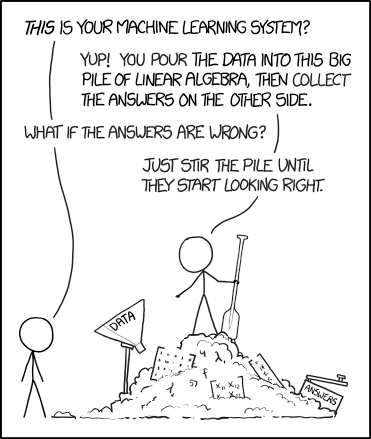
\includegraphics[height=0.55\textheight]{images/1838_machine_learning.png}
\end{column}
\begin{column}{0.50\textwidth}
\large
\textit{How do you teach a computer to \textbf{understand words}?}

\vspace{6mm}
Today: \textbf{Word Embeddings} --- turning text into numbers that capture meaning.
\end{column}
\end{columns}
\bottomnote{XKCD \#1838 by Randall Munroe (CC BY-NC 2.5)}
\end{frame}

% Slide 3: Learning Objectives
\begin{frame}{What You Will Learn Today}
\begin{enumerate}
\setlength{\itemsep}{8pt}
\item \textbf{Explain what word embeddings do} --- in plain English
\item \textbf{Show why simple numbering fails} and embeddings succeed
\item \textbf{Use embeddings for real finance tasks}
\end{enumerate}
\bottomnote{Everything is explained with pictures and analogies.}
\end{frame}

% Slide 4: TikZ Comic C1 --- "Lost in Translation"
\begin{frame}{The Problem: Computers Don't Understand Words!}
\centering
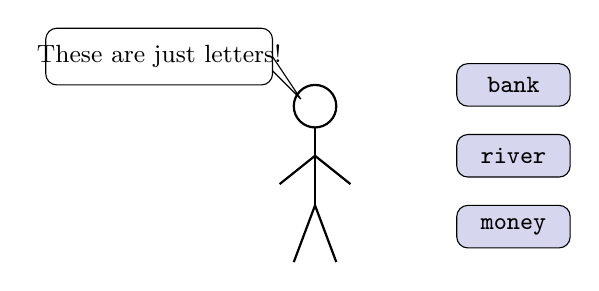
\begin{tikzpicture}[scale=0.9]
% Stick figure
\draw[thick] (0,2.2) circle (0.3);
\draw[thick] (0,1.9) -- (0,0.8);
\draw[thick] (0,1.5) -- (-0.5,1.1);
\draw[thick] (0,1.5) -- (0.5,1.1);
\draw[thick] (0,0.8) -- (-0.3,0);
\draw[thick] (0,0.8) -- (0.3,0);
% Word cards
\draw[fill=mllavender4, rounded corners] (2.0,2.2) rectangle (3.6,2.8);
\node at (2.8,2.5) {\small\texttt{bank}};
\draw[fill=mllavender4, rounded corners] (2.0,1.2) rectangle (3.6,1.8);
\node at (2.8,1.5) {\small\texttt{river}};
\draw[fill=mllavender4, rounded corners] (2.0,0.2) rectangle (3.6,0.8);
\node at (2.8,0.5) {\small\texttt{money}};
% Speech bubble
\draw[fill=white, rounded corners] (-3.8,2.5) rectangle (-0.6,3.3);
\draw (-0.6,2.7) -- (-0.2,2.3) -- (-0.6,2.9);
\node at (-2.2,2.9) {\small These are just letters!};
\end{tikzpicture}

\vspace{2mm}
A computer sees text as a string of characters. It has no concept of meaning.
\bottomnote{Computers need numbers, not words. But which numbers capture meaning?}
\end{frame}

% Slide 5: Why Not Just Number Words?
\begin{frame}{Why Not Just Number Every Word?}
\begin{columns}[T]
\begin{column}{0.47\textwidth}
\textcolor{mlred}{\textbf{Simple Numbering}}
\begin{compactlist}
\item cat = 1, dog = 2, car = 3
\item dog is NOT ``between'' cat and car
\item Numbers imply an order that doesn't exist
\end{compactlist}
\end{column}
\begin{column}{0.47\textwidth}
\textcolor{mlgreen}{\textbf{Embeddings}}
\begin{compactlist}
\item cat = [0.9, 0.1]
\item dog = [0.8, 0.2]
\item car = [0.1, 0.7]
\end{compactlist}
\vspace{2mm}
cat and dog are close (both animals). car is far away (different concept).
\end{column}
\end{columns}
\vspace{3mm}
\begin{block}{Key Insight}
Embeddings capture relationships. Simple numbers don't.
\end{block}
\bottomnote{Embeddings are learned from data --- the computer discovers which words are similar by seeing them in context.}
\end{frame}

% Slide 6: CHART --- Word Embedding Space
\begin{frame}{Words Can Become Points in Space!}
\centering

\includegraphics[width=0.65\textwidth]{01_word_embedding_space/chart.pdf}
\begin{compactlist}
\item Each word is placed at a specific location (coordinates)
\item Similar words end up close together
\item The computer learned these positions from reading text
\end{compactlist}
\bottomnote{Word embeddings turn words into vectors --- lists of numbers that capture meaning.}
\end{frame}

% Slide 7: TikZ Comic C2 --- "Words as Addresses"
\begin{frame}{Embeddings = Giving Words a Home Address}
\centering
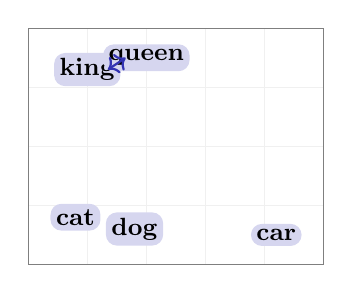
\begin{tikzpicture}[scale=0.75]
% Grid
\draw[step=1, lightgray, thin] (0,0) grid (5,4);
\draw[mlgray] (0,0) rectangle (5,4);
% Word labels at positions
\node[fill=mllavender4, rounded corners, inner sep=2pt] at (1.0,3.3) {\small\textbf{king}};
\node[fill=mllavender4, rounded corners, inner sep=2pt] at (2.0,3.5) {\small\textbf{queen}};
\draw[<->, mlpurple, thick] (1.35,3.3) -- (1.65,3.5);
\node[fill=mllavender4, rounded corners, inner sep=2pt] at (0.8,0.8) {\small\textbf{cat}};
\node[fill=mllavender4, rounded corners, inner sep=2pt] at (1.8,0.6) {\small\textbf{dog}};
\node[fill=mllavender4, rounded corners, inner sep=2pt] at (4.2,0.5) {\small\textbf{car}};
\end{tikzpicture}

\vspace{2mm}
Similar words live in the same neighborhood.
\bottomnote{In a city, nearby addresses mean nearby locations. In embeddings, nearby vectors mean similar meanings.}
\end{frame}

% Slide 8: CHART --- Word Analogy
\begin{frame}{The Magic of Word Math!}
\centering

\includegraphics[width=0.60\textwidth]{top10_08_word_analogy/chart.pdf}
\begin{compactlist}
\item King $-$ Man $+$ Woman $=$ Queen
\item Paris $-$ France $+$ Germany $=$ Berlin
\item Embeddings capture analogies as vector arithmetic
\end{compactlist}
\bottomnote{This is the ``aha moment'' of embeddings: meaning has direction. Gender, country, tense --- all are vectors.}
\end{frame}

% Slide 9: How Embeddings Are Made (TikZ flowchart)
\begin{frame}{How Embeddings Are Made}
\centering
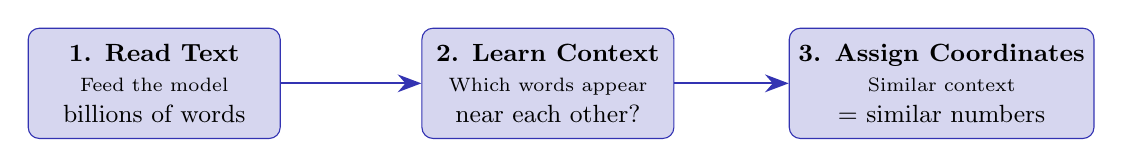
\begin{tikzpicture}[
  box/.style={draw=mlpurple, fill=mllavender4, rounded corners, minimum width=3.2cm, minimum height=1.4cm, align=center, font=\small},
  arr/.style={-{Stealth[length=3mm]}, thick, mlpurple}
]
\node[box] (a) at (0,0) {\textbf{1. Read Text}\\\scriptsize Feed the model\\billions of words};
\node[box] (b) at (5,0) {\textbf{2. Learn Context}\\\scriptsize Which words appear\\near each other?};
\node[box] (c) at (10,0) {\textbf{3. Assign Coordinates}\\\scriptsize Similar context\\= similar numbers};
\draw[arr] (a) -- (b);
\draw[arr] (b) -- (c);
\end{tikzpicture}

\vspace{5mm}
That's it. The computer reads text and figures out which words are similar.
\bottomnote{Word2Vec, GloVe, and BERT all follow this principle: learn from context.}
\end{frame}

% Slide 10: CHART --- Similarity Heatmap
\begin{frame}{Who Is Similar to Whom?}
\centering

\includegraphics[width=0.60\textwidth]{02_similarity_heatmap/chart.pdf}
\begin{compactlist}
\item Dark squares = highly similar words
\item Light squares = unrelated words
\item The computer learned this from reading text alone --- no human labeled it
\end{compactlist}
\bottomnote{Cosine similarity measures the angle between two word vectors. Small angle = similar meaning.}
\end{frame}

% Slide 11: CHART --- Embedding Neighbors
\begin{frame}{What Words Live Nearby?}
\centering

\includegraphics[width=0.60\textwidth]{top10_13_embedding_neighbors/chart.pdf}
\begin{compactlist}
\item Shows the closest words to a query word
\item Validates that the embedding captured real meaning
\item Similar words = similar contexts in training data
\end{compactlist}
\bottomnote{The nearest-neighbor test is a quick way to check if embeddings captured meaning.}
\end{frame}

% Slide 12: CHART --- Word Analogy Arithmetic
\begin{frame}{Vector Math Preserves Meaning}
\centering

\includegraphics[width=0.60\textwidth]{11_word_analogy_arithmetic/chart.pdf}
\begin{compactlist}
\item Visual proof that vector math preserves relationships
\item Directions in the space encode concepts like gender and geography
\item Not magic --- learned from co-occurrence patterns
\end{compactlist}
\bottomnote{Analogy arithmetic works because embeddings encode relational structure.}
\end{frame}

% Slide 13: Finance Application
\begin{frame}{Why Bankers Care About Embeddings}
\begin{compactlist}
\item \textbf{Sentiment Analysis}: Is this news article positive or negative for the stock?
\item \textbf{Fraud Detection}: Does this transaction description look suspicious?
\item \textbf{Document Search}: Find contracts similar to this one
\end{compactlist}
\vspace{3mm}
\begin{block}{Bottom Line}
Embeddings let machines understand financial text --- reports, news, filings.
\end{block}
\bottomnote{JPMorgan, Goldman Sachs, and Bloomberg all use NLP with embeddings for financial analysis.}
\end{frame}

% Slide 14: Try It Yourself
\begin{frame}{Try It Yourself: 3 Lines of Python}
\vspace{2mm}
\footnotesize
\texttt{from gensim.models import Word2Vec}\\[2pt]
\texttt{model = Word2Vec(sentences, vector\_size=100)}\\[2pt]
\texttt{similar = model.wv.most\_similar("bank")}

\vspace{5mm}
\normalsize
That's it --- three lines to train word embeddings on your own text.
\bottomnote{pip install gensim. For pre-trained embeddings, try gensim.downloader.}
\end{frame}

% Slide 15: TikZ Comic C3 + Key Takeaways
\begin{frame}{The Computer Gets It!}
\centering
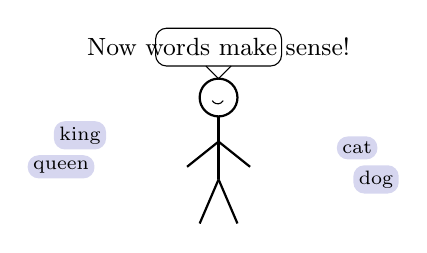
\begin{tikzpicture}[scale=0.8]
% Word clusters (left)
\node[fill=mllavender4, rounded corners, inner sep=2pt, font=\scriptsize] at (-2.2,1.0) {king};
\node[fill=mllavender4, rounded corners, inner sep=2pt, font=\scriptsize] at (-2.5,0.5) {queen};
% Word clusters (right of figure)
\node[fill=mllavender4, rounded corners, inner sep=2pt, font=\scriptsize] at (2.2,0.8) {cat};
\node[fill=mllavender4, rounded corners, inner sep=2pt, font=\scriptsize] at (2.5,0.3) {dog};
% Stick figure (center, happy)
\draw[thick] (0,1.6) circle (0.3);
\draw (-.1,1.55) arc (210:330:0.1); % smile
\draw[thick] (0,1.3) -- (0,0.3);
\draw[thick] (0,0.9) -- (-0.5,0.5);
\draw[thick] (0,0.9) -- (0.5,0.5);
\draw[thick] (0,0.3) -- (-0.3,-0.4);
\draw[thick] (0,0.3) -- (0.3,-0.4);
% Speech bubble
\draw[fill=white, rounded corners] (-1.0,2.1) rectangle (1.0,2.7);
\draw (-0.2,2.1) -- (0,1.9) -- (0.2,2.1);
\node[font=\small] at (0,2.4) {Now words make sense!};
\end{tikzpicture}

\vspace{2mm}
\begin{enumerate}
\setlength{\itemsep}{3pt}
\item Embeddings turn words into numbers that capture meaning
\item Similar words get similar numbers
\item Finance uses: sentiment, fraud detection, document search
\end{enumerate}
\bottomnote{Embeddings: giving every word a home address in number space.}
\end{frame}

% Slide 16: XKCD Closing
\begin{frame}{Go Teach a Machine Something}
\centering
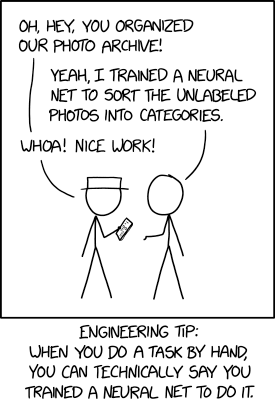
\includegraphics[height=0.55\textheight]{images/2173_trained_a_neural_net.png}
\bottomnote{XKCD \#2173 by Randall Munroe (CC BY-NC 2.5). Next: try the Jupyter notebook with real financial text data!}
\end{frame}

\end{document}
